%===============================================================================%
\chapter{Review of Literature}\label{chapter:literature}
%===============================================================================%

Understanding the scale, nature and dynamics of distribution of population across space and time has been the central premise of academic research in various fields of study such as human geography, sociology, transportation, urban planning and managements.
This granular knowledge of where people are and how they move is also critical in practical decision making in various industries such as real estate for valuing places, retail for business planning and risk management during emergencies for evacuation.
The primary challenge faced by any research concerning the population at this scale is the collection of precise and accurate data in a timely manner.
Though large structured datasets such as national census provides comprehensive coverage they are sparse temporally and understanding dynamics of population withing shorter periods is not possible.
Alternatively, smaller datasets such as sample surveys and traffic counts are collected more frequently they are not comprehensive enough. 
This pursuit for identifying a data source which has the best features of both type of datasets started as an inquiry into methods to estimate and interpolate highly granular data from existing regional level aggregate data.
As technology improved through the later half of twentieth century, research methodologies adopted the new tools and technologies to not only improve the quality of estimations but also to collect data with high granularity.
Though new technologies provided immense opportunity in collecting large amounts of data which were previously impossible, they also introduced their own share of uncertainties.
Hence it becomes imperative that we understand the evolution of these techniques and methodologies along with the research that used them to build our rationale behind any further research.
Moreover with the proliferation of mobile devices and wireless internet connectivity, every day to day activity is being digitised leading to the creation of large amount of easily accessible data which are generated passively in an unstructured manner.
The users' acceptance to the collection and analysis of such data has also been improving until recently \cite[-2cm]{kobsa2014}.
There has also been rising concerns regarding user privacy along with the development of more accurate methods to track them.
In this context, the critical task in all these research is to solve the problem of balancing these two - collecting relevant data and protecting user privacy, by choosing the right technologies and devising the appropriate methods.

In this chapter a systematic survey of literature in the broad multidisciplinary area of research - `distribution and dynamics of human activity' has been conducted.
The aim of this survey was to evaluate the stage at which the research is currently at, understand its evolution and progress through time and identify the possibilities that exists for future research.
A comprehensive survey of over 300 publications which discuss this area of research was undertaken covering the major themes and trends in the last 70 years.
These themes were discussed in detail to outline what has been achieved in the corresponding fields of study highlighting the opportunities and gaps in research that still exist.
The timeline of publication of these research has also been studied to discuss the evolution of the research along with the changes in the technology landscape.
These studies were then classified in terms of the major technologies employed by them to uncover the trends in how various technologies have been adopted and phasing out during this period.
The primary objective was to understand the advantages and disadvantages of these techniques and to develop a theoretical framework for understanding when and how to use them effectively to answer research questions.
Finally the literature survey was summarised focussing on the major research gaps that still exist and interesting new areas of research that has emerged recently  where more research is warranted.
These areas of research were also critically evaluated in terms of priority and feasibility leading to the development of questions and plan for this research thesis. 

\begin{marginfigure}
  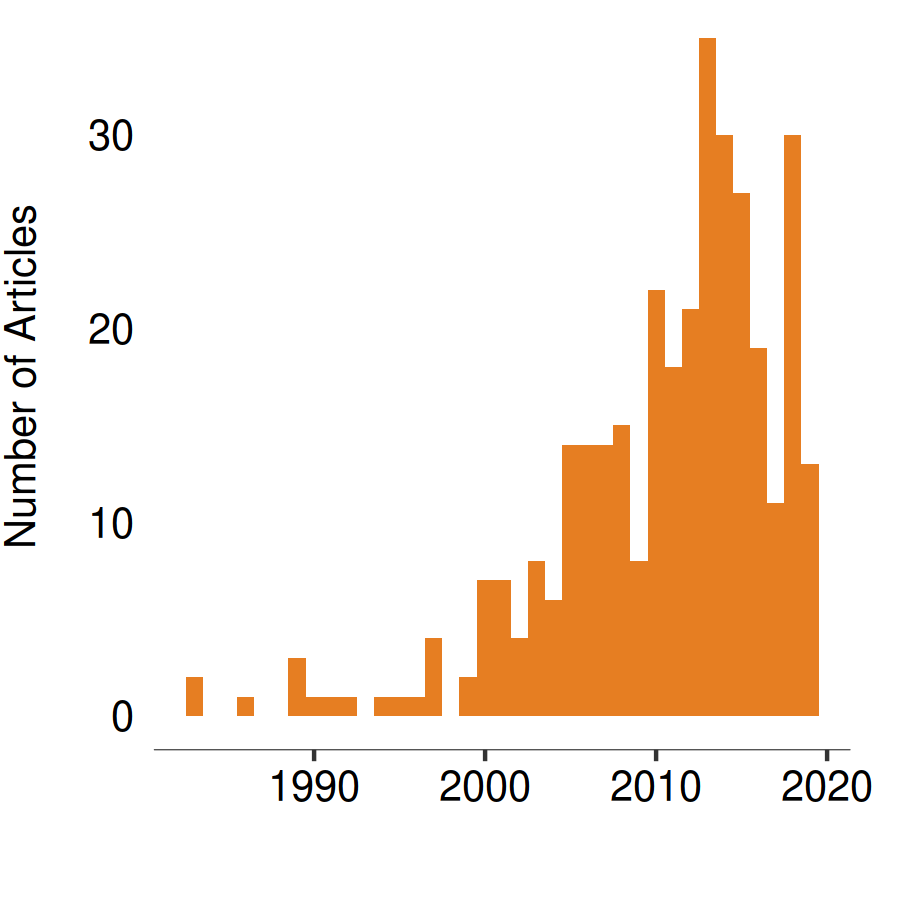
\includegraphics{images/literature-timeline.png}
  \caption{Growth of research in the area of 'Understanding distribution and dynamics of human activity' since 1980}
  \label{figure:literature:timeline}
  \vspace{1em}
  \noindent\fontsize{7}{7}\textit{Measured in the number of papers published}
\end{marginfigure}

The set of works which discuss the use of mobile devices based technologies for studying topics in disciplines such as geography \citet{li2016}, urban analysis \citep{ratti2006}, urban computing \citep{jiang2013} and other general applications and opportunities \citep{steenbruggen2013, arribas-bel2014}, serve as our starting point for this literature survey.
The search was then expanded from these reviews by navigating through their citation networks and identifying further research that are relevant.
Though this did not provide a perfectly comprehensive set of literature, it did provide a representative sample of all the different disciplines and directions of the research conducted in the area.
Through this process, around 325 relevant research publications were identified which dealt with the collection, measurement, analysis, visualisation and discussion of population and their movement at a granular level.
Research in this area started around 1950s where possibility of estimating day-time urban population at a granular level using existing  broader data employing various estimation methods were discussed \cite{foley1954, schmitt1956}.
Though this served as a starting point, the pursuit of such granular data and their applications in corresponding fields didn't pick up until the start of the 21st century during the `digital revolution' when personal computing become mainstream which was followed by the growth of internet.
Figure \ref{figure:literature:timeline} shows the yearly volume of research published since 1980 from which it can be observes that though there were some research conducted through 80s and 90s the real push forward came around beginning of the millennium when mobile phones adoption skyrocketed.
In addition to the early 2000s, a substantial increase in interest can also be seen in the beginning of the next decade fuelled by the smartphone revolution which completely changed the research avenues in-terms of volume and types of data available and methodologies available to tackle them.
While the mobile phone era put a device in every ones pockets, the smart phone era has armed them with immense data collection capabilities.
The area of research is multidisciplinary encompassing academic interest and commercial applications in various disciplines and industries spanning across wide range of themes as discussed in section \ref{section:literature:themes}.

%-------------------------------------------------------------------------------%

%==============================================================================%
% Section Introduction
%==============================================================================%

\section{Research Themes}
In this section we look at the major themes and questions tackled by this knowledge base.
We start by classifying the research into the major and minor themes explored in them as shown in Figure \ref{figure:literature:themes}.
The tree-map shows the volume of research in corresponding themes measured in terms of number of publications.
We can observe that the research is conducted in five major areas - population studies focussing on the creating and utilising data on distribution and nature of human activity, mobility and interaction focussing on the changes in these distributions, understanding the nature and function of space from these distribution and change, methods and techniques which can be used to conduct the research and finally issues and solutions related to the privacy of the users while conducting these research.
We can also observe that most of the research apart from developing methods were conducted in the domain of human mobility and social interaction closely followed by the population distribution.
In the following sections we discuss these in detail along with their sub themes with the following framework,

\begin{enumerate}
  \setlength{\itemindent}{2em}
  \itemsep-0.25em
  \item What are the major lines of questioning?
  \item What has been done previously?
  \item Where are the opportunities for further research?
\end{enumerate}

\begin{figure}
  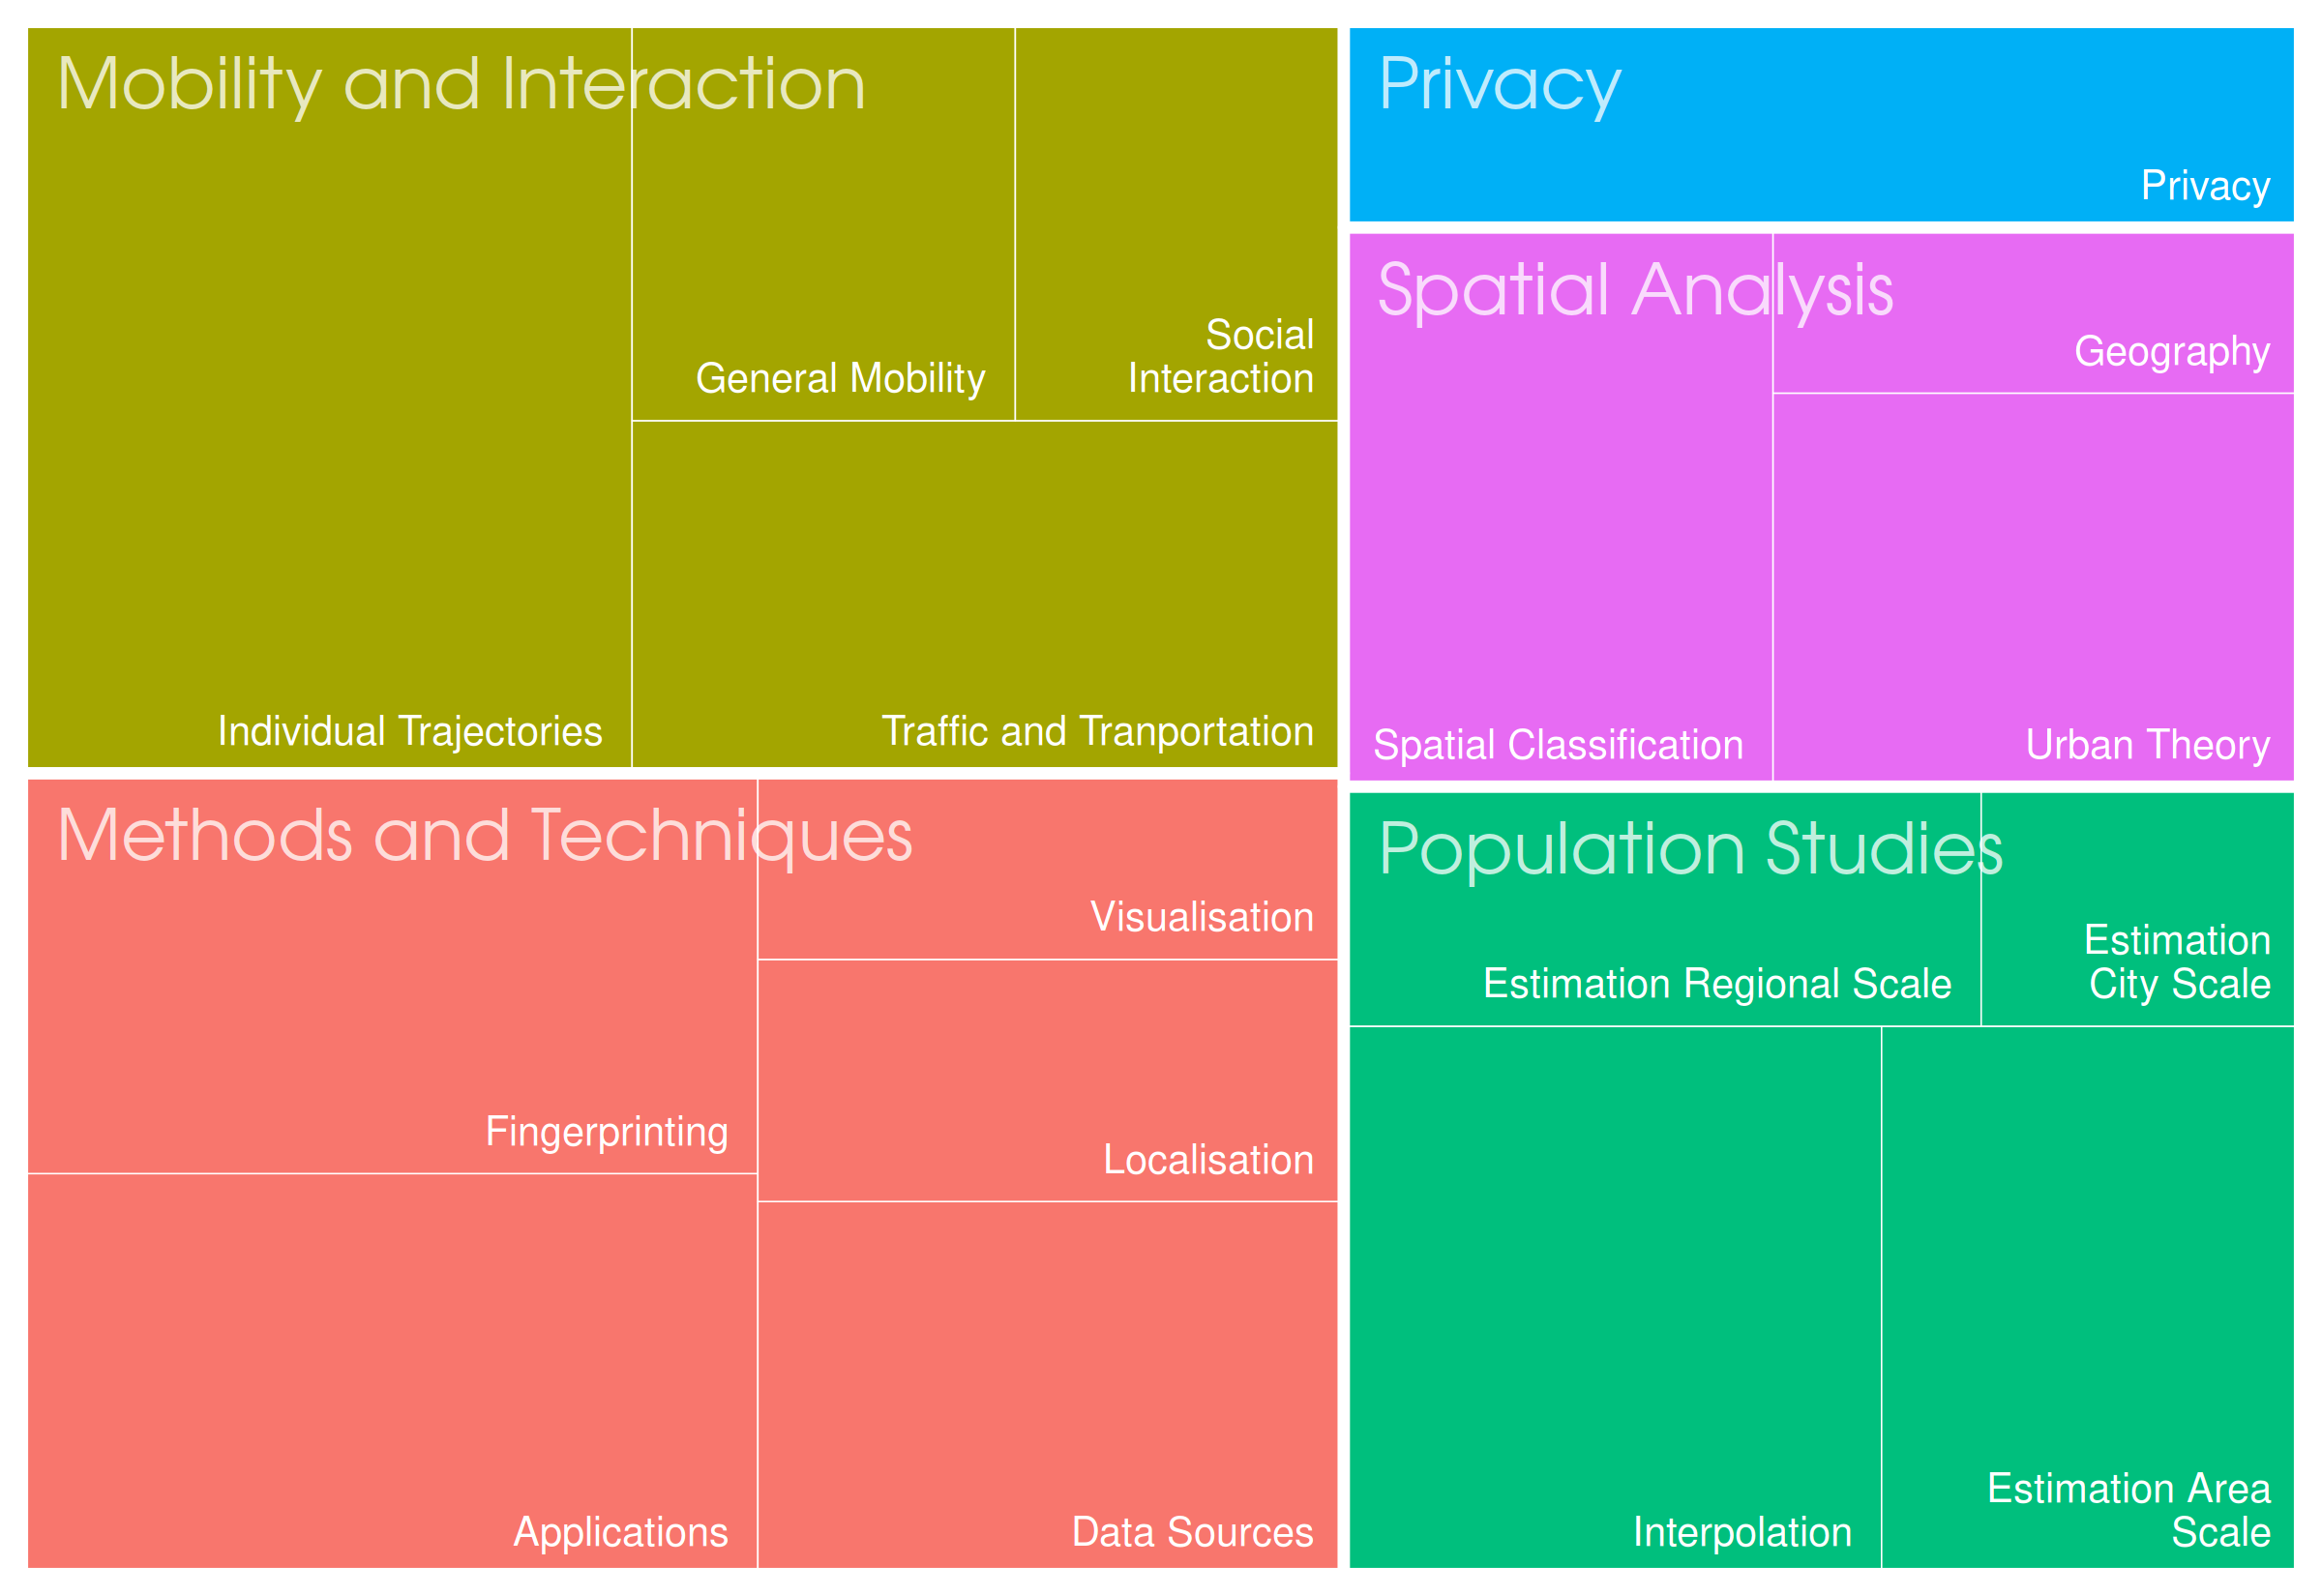
\includegraphics{images/literature-themes-treemap.png}
  \caption{Tree-map showing the volume of research conducted under each major themes and their sub-themes.}
  \label{figure:literature:themes}
\end{figure}

%------------------------------------------------------------------------------%
% Population Studies
%------------------------------------------------------------------------------%

\subsection{Population Studies}
Though \citet{foley1954} and \citet{schmitt1956} started this line of research in 1950's with the discussion on estimating daytime population using broader datasets it was not until the 80s significant volume of research kicked off in this area of study.
From 80s until mid 2000's numerous studies were conducted on measuring and studying the population at a granular level both spatially and temporally.
The focus of the research around this time was primarily on interpolation from the larger datasets created using censuses, regional or national level sample surveys and other centrally collected sources of data.
There have been numerous fairly successful attempts with methodologies where a broad dataset such  as regional level population summaries and modelling or interpolating more granular data from them by augmenting with other sources of data such as street networks \citep{reibel2005}, remote sensing \citep{sutton1997, yuan1997, chen2002} etc.
\citet{dobson2000, dobson2003a, bhaduri2002, bhaduri2007} and \citep{mennis2003, mennis2006} are examples of such research methodology.
These studies were almost done on a city scale or above with mostly modelling or interpolation methods since the data sources were few and were centrally collected.

Around 2005, there was a sharp shift in research where the interpolation methods were replaced by highly available granular data collected over cellular network.
Studies were conducted on estimating population densities, presence of tourists, general activity pattens using data from cellular networks.
Most of these research were conducted at a far larger geographic scale looking at things at an area level \citep{pulselli2008,girardin2009,phithakkitnukoon2010,yuan2016}.
There were efforts in using device level sensors such as global positioning system(GPS), Wi-Fi and Bluetooth to detect population distribution and socio-geographic routines \citep{calabrese2010,rose2010,farrahi2010}.
There have been studies on looking at people distribution as granular as queue lengths as discussed by \citep{wang2013} to city level dynamic population mapping where the limitations of traditional datasets generated through censuses and surveys \cite{deville2014}.

Around the 2015, along with the data collected directly from the mobile devices,the data that are generated by the users activity on these devices are became more important.
Social media data such as twitter \citep{lansley2016} and other consumer data such as loyalty cards \citep{lloyd2018}, smart cards \citep{ordonez2012} etc. have also become a significant sources of data for such research.
Recently, with increased concerns and legislation on privacy, there have been studies which go back to the effort of interpolating granular data from broader datasets but using more data and processor intensive technologies such as agent based modelling, deep learning, small area estimation \citep{crols2019, shibata2019, rao2015} etc..
Though there have been a lot of work done in most of the directions in this research area, the clear gap arises due to the absence of a continuous, granular and sufficiently longitudinal data-sets to complement the methodologies that have been developed. 

%------------------------------------------------------------------------------%
% Mobility and Interaction
%------------------------------------------------------------------------------%

\subsection{Human Mobility and Interaction}

This is one of the major areas of research which have significantly benefited from the decentralised collection of data at a granular level \cite{castells2000}.
In addition to being useful in their own right, these data were in turn used to augment traditional models of travel behaviour, traffic and transport to provide a better understanding of human movement over time and space \citep{janssens2013}.
The major themes of research within this area are, Movement of people in space and time with emphasis on understanding the built environment, social interaction between these people with a sociology perspective and traffic and transportation studies with a infrastructure perspective.
There is significant volume of research which dealt with recording and analysing the trajectories of the users to understand their movement patterns enabled by the unprecedented availability of detailed data from mobile devices.

% \begin{enumerate}
%   \setlength{\itemindent}{2em}
%   \itemsep-0.05em
%   \item 
%   \item 
%   \item 
% \end{enumerate}

%------------------------------------------------------------------------------%
% Methodology and Techniques
%------------------------------------------------------------------------------%

\subsection{Methodology and Techniques}

\citep{maceachren2001}
\citep{hallisey2005}
\citep{morrison2000}
\citep{lobben2003}
\citep{harrower2007}
\citep{ferrara2014}
\citep{fabrikant2005}
\citep{thomas2005}

Visualising the temporal dynamics of data collected on human activities through decentralised processes poses significant challenges when approached with traditional cartographic concepts (MacEachren, 2001 Hallisey, 2005).
Digital media especially animation has been explored as an option to solve for the temporal dimension (Morrison, 2000; Lobben, 2003) but is bound by the cognitive limits of the viewer (Harrower, 2007).
There have been approaches proposed around animations of generated surfaces (Kobayashi, 2011) and network-based visualizations (Ferrara, 2014) leaving gaps in research for new methods in dynamic geographic visualisation (Fabrikant, 2005) and visualising path and flow of phenomena (Thomas, 2005).
This provides us with a promising opportunity for research in methods for visualising high frequency, hyper-local pedestrian data within the limits of cognition of the viewer.

%------------------------------------------------------------------------------%
% Spatial Analysis Theory and Modelling
%------------------------------------------------------------------------------%
\subsection{Spatial Analysis - Theory and Modelling}

Traditional and modern geography was dominated by the study of centrally collected data acquired through extensive field surveys and remote sensing.
In the last two decades, a significant paradigm change has been introduced by the availability of unprecedented amount of data generated by unconventional sources such as mobile phones, social media posts etc.
This move to the postmodern geography has been accompanied by a change in our understanding of the built environment and human geography from a static point of view to a more dynamic definition \cite{soja1989}.
This definition is based on the bottom-up mechanisms which make human activity such as information exchange and economy to manifest in the physical built environments as argued by \citep{batty1990, batty1997, batty2012} and \citep{batty2013, batty2013a}.

This transition into the digital age \citep{graham1999, tranos2012, tranos2013} has changed the politics of space and time \citep{massey1992} and been more pronounced in the study of urban built environment where technology has redefined the concepts of place and space \citep{graham2001, graham2002, sassen2001}.
With the ability to collect and analyse of data on large complex systems in real-time \citep{graham1997}, we are exploring the possibilities of understanding their structure and organisation using concepts of complexity theory \citep{bettencourt2013, portugali2012} with more emphasis on their temporal patterns such as the argument towards finding the pulse of the city \citep{batty2010}.
With the population getting more and more connected \citep{castells2010}, the nature of space/place is being dynamically defined by the population themselves \citep{giuliano1991} and vice versa \citep{zandvliet2006}.
This flood of hard data \cite{nature2008} was accompanied not only by optimism in its potential \citep{thomas2001} but also by the questions raised on the challenges in handling the diverse, large scale, non standardised data it produces and the usefulness or representativeness of the resulting analysis \citep{miller2010, arribas-bel2014a}.

However, availability of such data has impressive uses in urban studies \citep{bettencourt2014} especially with advancement of new technologies \citep{steenbruggen2015} and possibility of distributed, crowdsourced data collection \citep{lokanathan2015}.

%------------------------------------------------------------------------------%
% Privacy
%------------------------------------------------------------------------------%
\subsection{Privacy}

The ubiquity of personal devices and digitisation of day to day activities through these mobile devices \citep{mcmeel2018dark} has provided many opportunities for researchers and industry for collecting, analysing and deriving inputs from them.
However at the same this also increased the risk of infringement on privacy of the users whose data is being collected \cite{saponas2007, krumm2009}.
There is immense value in uniquely identifying and profiling information on people for specialised purposes such as security \citep{cutter2006} and law enforcement \citep{dobson2003} but also has extreme risks associated when not handled with care \citep{vanwey2005}.

Strictly protecting personal information while ensuring the information is usable for research by maintaining the uniqueness in the data is the major concern which was addressed by devising frameworks for secure practices in confidentially collecting and using the location data \citep{duckham2006, tang2006, lane2014}.
Some efforts sought to accomplish this task through cryptographic hashing algorithms (Pang, 2007) while others aimed to thwart identification and tracking at the device level by techniques such as MAC randomisation \citep{gruteser2005, green2008}.
Finally though getting consent of users for the collection and use of such information from their mobile devices is challenging, there is a significantly improved acceptance when the process offers value in return such as discounts and monetary benefits \citep{kobsa2014user}.

There is opportunity in this area for research in applying the cryptographic solutions along with the privacy preserving frameworks to arrive at methods which can extract useful information out of large personal data while obscuring or anonymising them.

%==============================================================================%
% Research Trends
%==============================================================================%

\begin{figure*}
  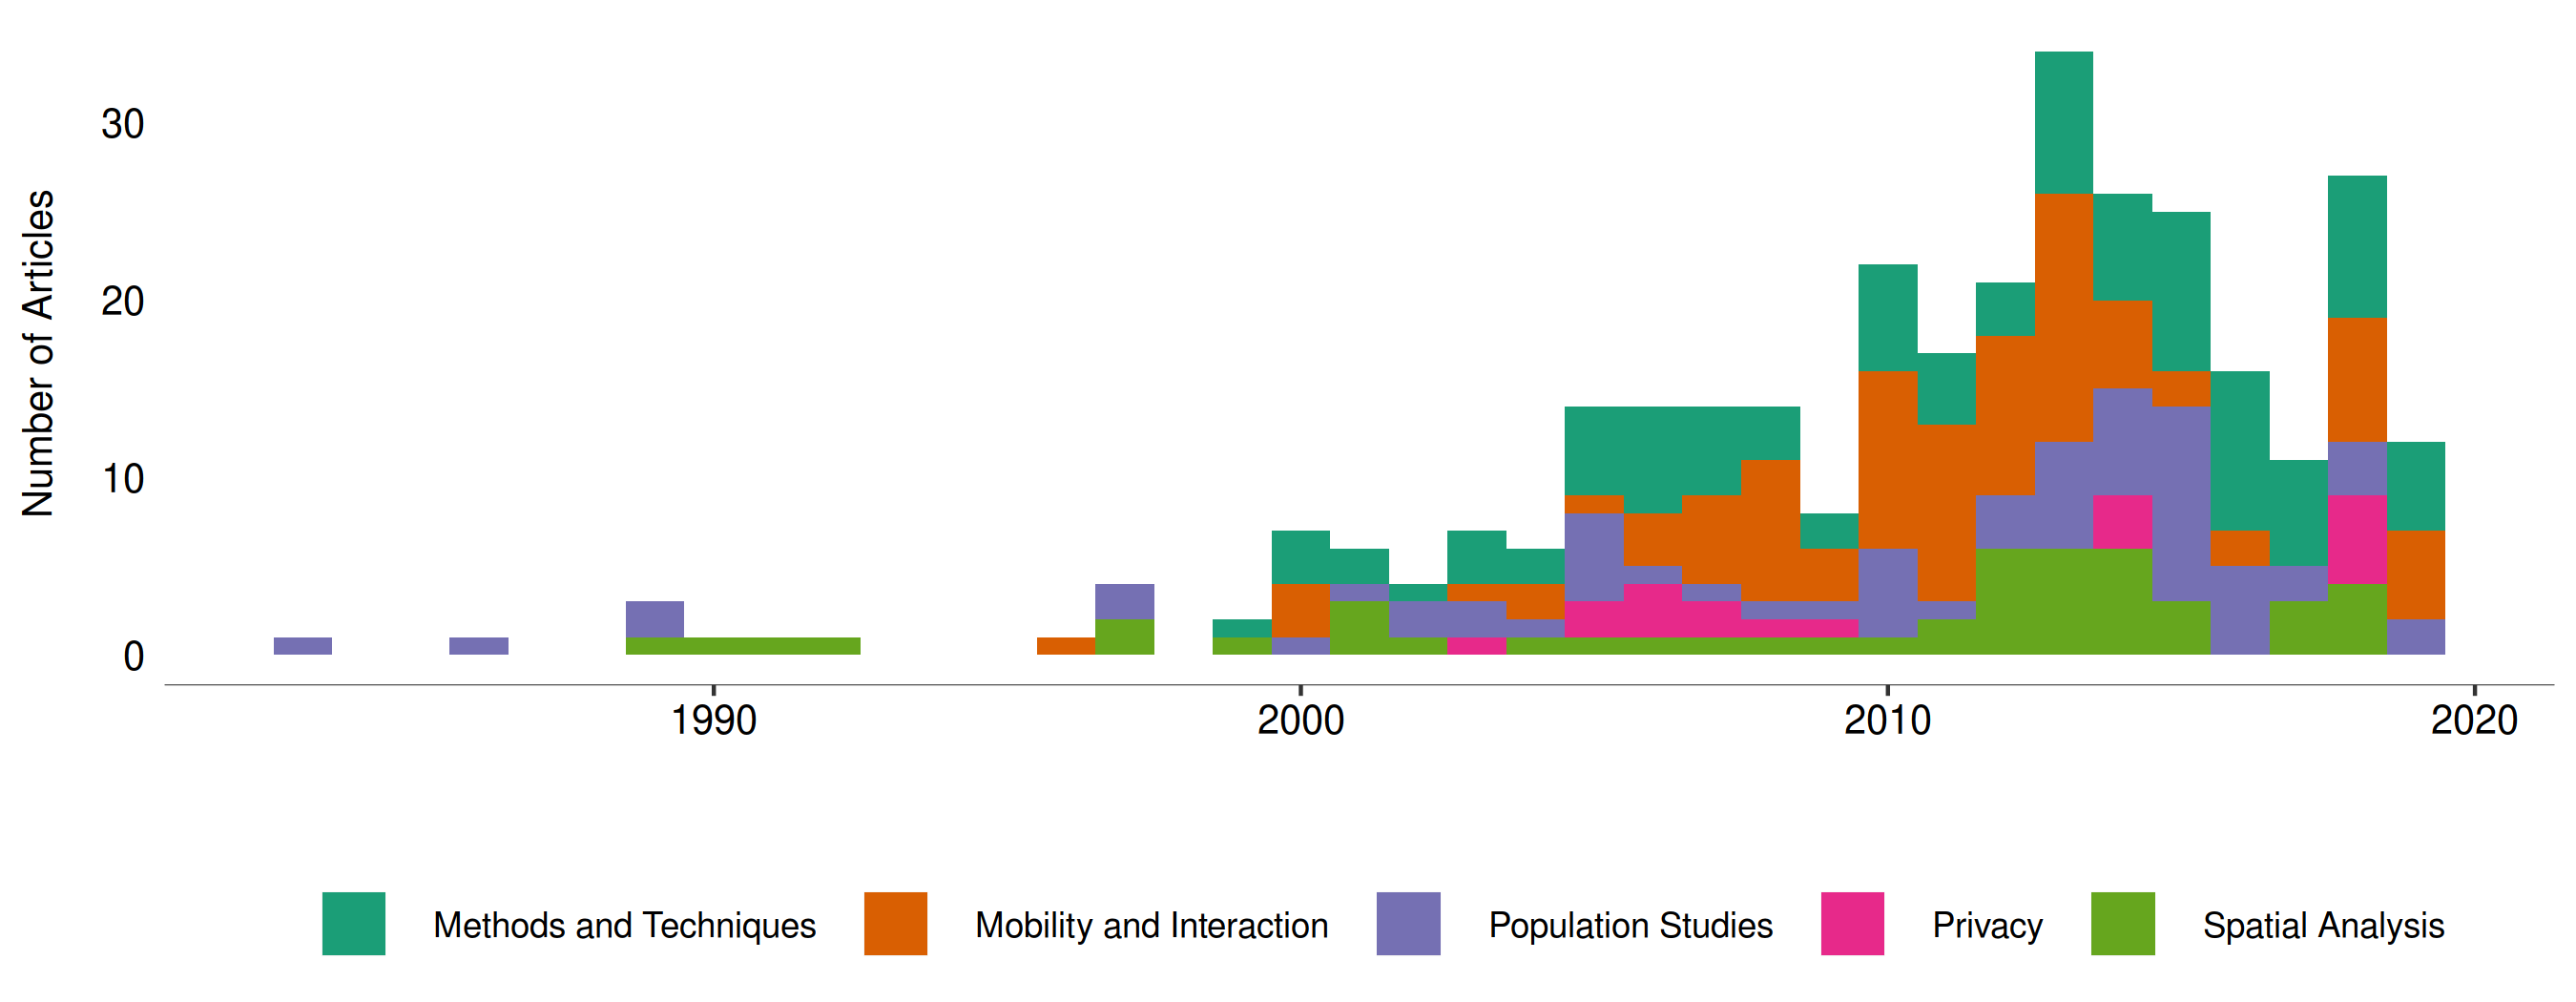
\includegraphics{images/literature-themes-timeline.png}
  \caption{Outline of the `Medium data toolkit' devised to collect, process, visualise and manage the Wi-Fi probe requests data}
  \label{figure:literature:themes:timeline}
\end{figure*}

\section{Research Trends}

Figure \ref{figure:literature:themes:timeline} shows the volume of research done in this topic since 1980 categorised based on their major themes discussed earlier.
We can observe that there are distinct trends in the research over time, which evolved around the development of technology in the last two decades.
Until 90s the research was mostly centered around population studies on estimating and interpolating granular spatial and temporal information from larger and cross sectional datasets such as census and sample surveys.
The period between 2000-2010 there was interest in potential of the new data generated by the digital revolution. 
We can categorise this as the `mobile era' where carrying mobile devices become mainstream.
This explosion of research coincided with mobile phones becoming more popular and ubiquitous with population in urban areas and was around development of methods and techniques to utilise the data generated from them.
There were also extensive studies in using the datasets to understand human mobility along with a rising concern in the privacy of the users who's data which are being used for these studies.

%------------------------------------------------------------------------------%

The release of iPhone in 2008 and the increase in the share of 'smartphones' in the next 10 years sparked the `smartphone' era. 
The change made sure that all the mobile devices gaining numerous capabilities such as internet connectivity over Wi-Fi and mobile network, location awareness with global positioning system, movement recognition with accelerometers and connectivity other `wearable' devices through Bluetooth.
This also lead to the digitisation of lifestyle where every aspect of the life being done through these devices over internet while generating huge amount of data on these activities.
This sparked the large volume of research on the form and function of space by studying this data and on the dynamics of human population in space and time in the next 5 years.
These research were particularly centered around tracking the trajectory of people using the mobile devices they carry with them as the smartphones made it easier to collect the necessary data directly from them rather than depending on a centrally collected datasets from mobile carriers. 
With the theoretical limit to predictability in human mobility quantified \cite{song2010limits}, the focus on urban mobility has been declining in the past few years which has led to a renewed interest in population studies at a local-local level in real-time.
In addition to using the data from the mobile devices, these studies have also been exploring the use of large assemblages of consumer data that are being generated in this connected mobile environment and linking them together to create a fuller picture \cite{cdrc2018}

%------------------------------------------------------------------------------%

Finally, with the increase in use of personal data, there has also been an increase in research regarding the privacy of the users.
Along with this, the mobile devices and subsequently the data generated by them are more and more anonymised so that the users cannot be tracked or identified at a personal level.
This has given rise to the new trend in research to devise methods to overcome this anonymisation and at the same time research which considers these methods as vulnerabilities and find solutions to make the anonymisation process more robust. 
There is clear need for methods which anonymise the data sufficiently to protect the identity of the users and at the same time enable us to conduct research in
measuring studying population distribution and movement at a granular level.

%==============================================================================%
 

%------------------------------------------------------------------------------%
\section{Techniques and technology}\label{section:literature:technology}
%------------------------------------------------------------------------------%

\begin{marginfigure}
  \forcerectofloat
  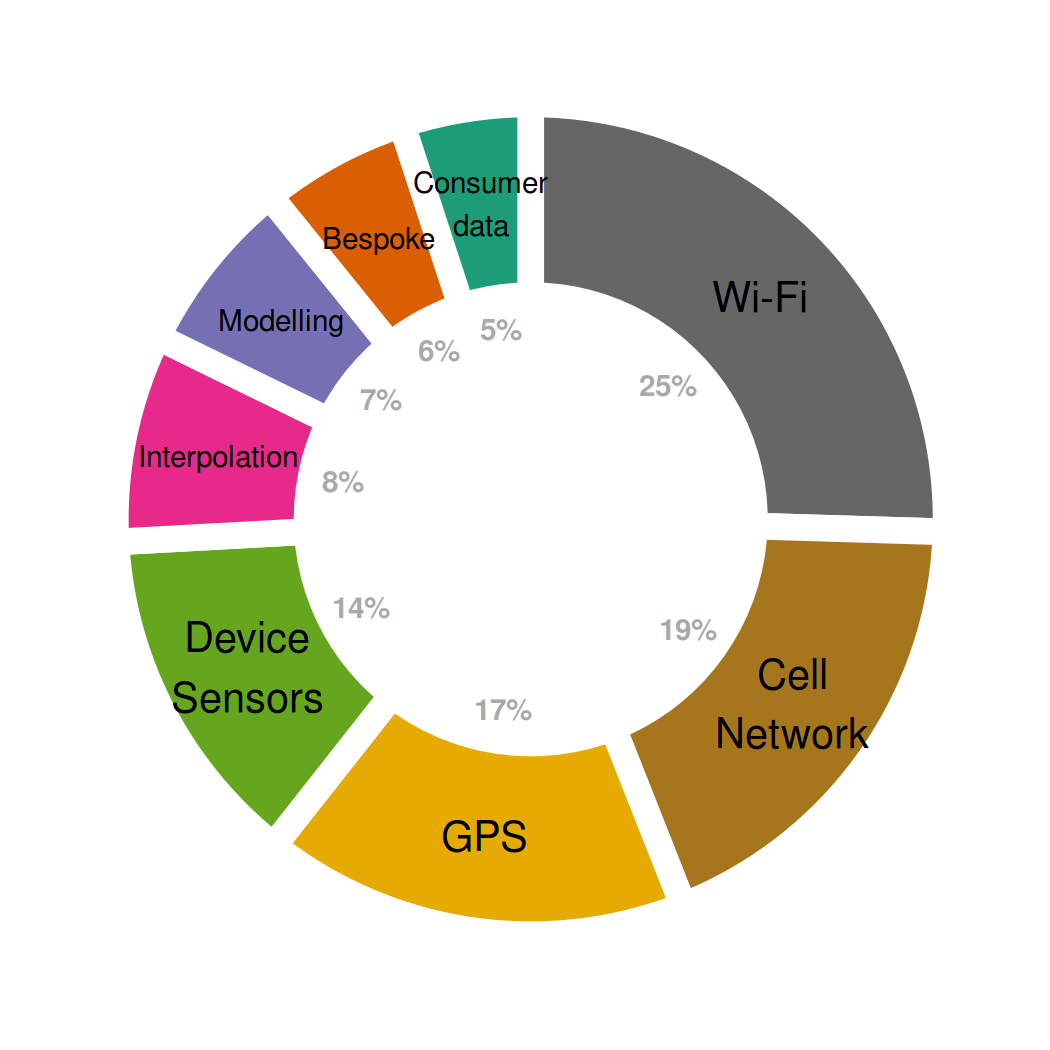
\includegraphics[trim={1.1cm 1cm 1cm 1cm},clip]{images/literature-technology.png}
  \caption{Distribution of research across various techniques and technologies}
  \label{figure:literature:timeline}
\end{marginfigure}
\marginnote{\noindent\fontsize{7}{7}\textit{Measured in the number of papers published}}

When we look at the literature from the technology perspective, we observe that over the years, the research continuously picks up and applies recent technological developments in the pursuit of understanding the distribution of human activity and population.
Figure \ref{figure:literature:timeline} shows the distribution of the research in terms of the main technique/ technology used over the past 40 years.
We observe that the earliest attempts started from the exploration of using interpolation and modelling techniques on a broader dataset.
As the need for more granular datasets increased there were attempts to devise and utilize bespoke solutions to generate them.
When mobile devices became mainstream, the focus shifted to utilize the relevant components of the mobile infrastructure.
A significant number of studies were done in utilising data collected from the mobile network, sensors in the mobile devices, especially GPS and Wi-Fi, in addition to the social media content generated from these devices.
A detailed account of these studies is given below,

\begin{figure*}
  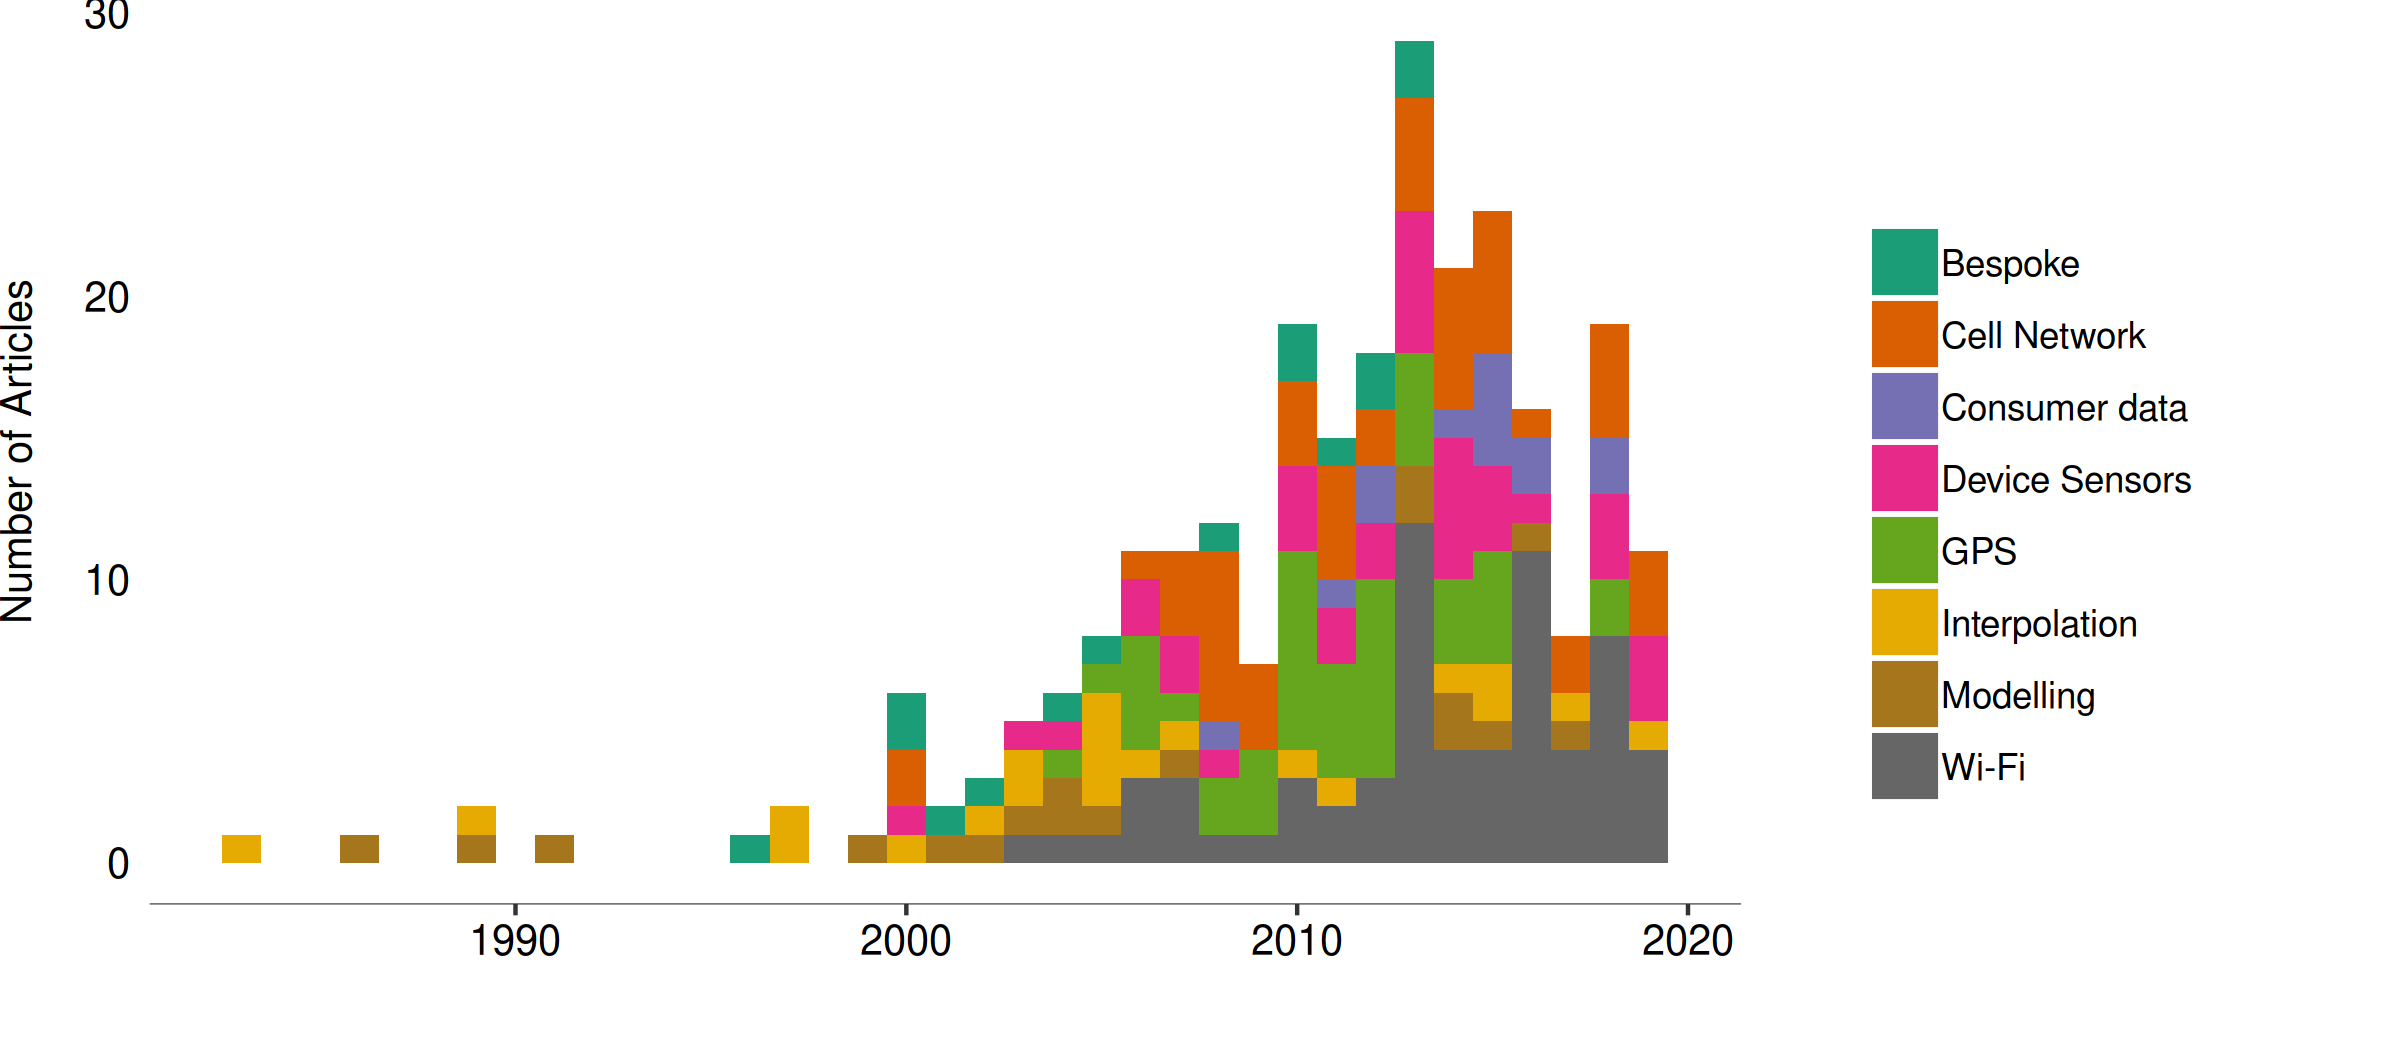
\includegraphics{images/literature-tech-timeline.png}
  \caption{The evolution of research since 1980 in terms of the the technology used in the research.}
  \label{figure:literature:tech:timeline}
\end{figure*}

%------------------------------------------------------------------------------%
\subsection{Interpolation and Modelling}
%------------------------------------------------------------------------------%

Attempts in using the existing data collected through traditional methods such as census and large scale sample surveys to create spatially and temporally granular and detailed estimates were carried out by applying various interpolation methods such as pycnophylactic, dasymetric interpolation \citep{tobler1979, mennis2003, mennis2006, hawley2005, tapp2010, wismans2017} along with spatial \citep{lam1983,martin1989, martin2015} and temporal interpolation techniques \citep{glickman1986}.
These methods along with supplementary data such as remote sensing imagery \citep{sutton2001, chen2002} and street networks \citep{reibel2005} were shown to be useful in producing detailed granular population maps at various scales with varying degree of success \citep{dobson2000, bhaduri2002, dobson2003, bhaduri2005, bhaduri2007}.
These approaches have been employed in various applications such as econometric studies \citep{mcdonald1989}, studies on public health \citep{hay2005}, emergency management \citep{kwan2005} and flood risk estimations \citep{smith2016}.

In addition to these interpolation techniques classic modelling techniques can also be used to estimate daytime populations and demographic structure at hyper-local scales \citep{jochem2013, jia2014}, urban scales \citep{alahmadi2013, abowd2004} and regional scales \citep{foley1954, schmitt1956, singleton2015, mccormack2017}.
The granular data created with such modelling techniques are shown to be useful in urban planning and management \citep{parrott1999}, emergency management \citep{alexander2002, cutter2006} and in modelling traffic and transportation \citep{lefebvre2013}.
These interpolation and modelling techniques along with granular data produced are also used in classifying spatial areas and hence understanding the structure of cities in general \citep{mcmillen2001, mcmillen2004, lee2007, arribas-bel2014}.
Though being useful, these techniques are still shown to have limitations and uncertainties \citep{nagle2014}, which mostly arise from the nature of the input data employed.
This leads us to the need for more detailed and frequent collection of data.

%------------------------------------------------------------------------------%
\subsection{Bespoke technologies}
%------------------------------------------------------------------------------%

Following this need, there has been efforts to use bespoke or specialised technologies such as cameras \citep{cai1996, heikkila2004, krockel2012}, Lasers \citep{zhao2005, arras2008} and radio frequency receivers  \citep{bahl2000, yang2013, chothia2010, bulusu2000, dil2011} to measure human activity.
But the major problem with such solutions is the cost and effort involved in designing and implementing them at urban and regional scales comprehensively.
Moreover, being specialised and centralised they tend to be challenging to maintain and update as the technological landscape change.
This gives us the need to identify and use techniques which are more general in nature and can be used for longer periods of time which are cheap to install to achieve a more comprehensive coverage.

%------------------------------------------------------------------------------%
\subsection{Cellular Network}
%------------------------------------------------------------------------------%

The rise of mobile phones as ubiquitous personal devices for the broader population has provided us with a viable alternative for collecting data with finer granularity at large scales.
Mobile infrastructure consists of both the `network part’, built and managed by the service providers, and the `user part’, which is the phones owned by the users’ themselves.
The network part, in addition to providing connectivity to the users, also collects information on these devices actively such as communication between the users and passively such as when the phones themselves move from tower to tower.
The mobile devices themselves have a variety of sensors such as accelerometer to identify movement, compass to identify orientation, GPS receiver to deduct geographic position, etc.
They also have various communication capabilities such as cellular, Wi-Fi, Bluetooth and Near field communications (NFC) etc. 
Both of these sensors and communication capabilities can be used as sources of data themselves.
With the growth of mobile devices and the infrastructure surrounding it, there has been significant effort in utilising data generated by every component of this complex infrastructure.

The first set of research started to use the cellular network data for urban studies \citep{jiang2013,steenbruggen2015, lokanathan2015, calabrese2015, reades2007}.
Even though this approach has been acknowledged to have inherent biases such as ownership bias across particular demographic groups \citep{wesolowski2013} the relative advantages such as coverage made them excellent sources of data.
Visual exploration of use of such data using interactive interfaces to evaluate quality of service and scenario testing has been tested for the optimisation of public transport \cite[-4cm]{sbodio2014}.
Such network data with the active and passive information collected from them can be used to create trajectories of people \cite{schlaich2010}, detect their daily routine \cite[2cm]{sevtsuk2010} and classify those routes in terms of function \citep{becker2011a}.
It was also demonstrated to be useful in understanding overall mobility and flow of people and information \citep{candia2008, krings2009, simini2012, zhang2019}.
These data can be used to identify asymmetry in flow of people spatially \citep{phithakkitnukoon2011}, estimate volume and pattern of road usage \citep{bolla2000, wang2012} and by augmenting the topology to optimise operations \citep{puzis2013}.
Such datasets have been extensively used in traffic and transportation research to derive origin-destination matrices \citep{caceres2007, mellegard2011, iqbal2014}, travel time estimation \citep{janecek2012} and traffic status estimation \citep{demissie2013, grauwin2015}. 

It has been shown that mobile network data can be used to uncover nature of the population such as tourists in specific areas \citep{girardin2008} and the interaction between the people in the study area \citep{campbell2008}.
The structure \citep{onnela2007, onnela2007a}, geography \citep{lambiotte2008} and dynamics \citep{hidalgo2008} of such networks have been studied and demonstrated to be useful in predicting their change \citep{wang2011, vajakas2018} over time.
This social networks and their spatio-temporal structure can also be used for classification of land use \citep{pei2014, jia2018}, assessment of spatial patterns \citep{reades2009, steenbruggen2013} and understanding the broader spatial structure of cities \citep{louail2014, arribas-bel2015} and regions \citep{arhipova2018}.
The data collected from the cellular network when examined at granular levels such as inter-personal communication and economic activity can be used to create estimations of micro area-level population density \cite[-4cm]{pulselli2008, ng2017} and also the characteristics \cite[1cm]{girardin2009} and the nature of the activity \citep{phithakkitnukoon2010}.
Aggregated human activity measured from such research in turn can be used to measure and model population dynamics and land use density and mix at broader level \citep{jacobs-crisioni2014, tranos2015, tranos2018}.
The spatial patterns thus uncovered can then be applied to urban planning \citep{becker2011b} whilst the temporal patterns uncovered have immense utility for the disciplines such as epidemiology.
For example, population influxes measured from changes in mobile network usage can be used to model spread of diseases \cite{buckee2015}.

Though the mobile network provides much more granular and accurate data than interpolation techniques, it is not without its limitations \citep{yucel2017}.
The distribution of network infrastructure usually follows the purposes of service coverage and follows commercial decisions. 
This introduces systematic biases in the data passively collected through them.
Moreover, the data actively collected through them has bias based on the volume of usage of services by the customers which can vary widely spatially, temporally and also based on demography.
In addition to this because of the coverage, the data collected from mobile service providers pose immense privacy risk when linked to other sources of consumer data.
This makes collection of data directly from the devices using the sensors on the device much more robust in certain cases.

%------------------------------------------------------------------------------%
\subsection{Mobile Sensors}
%------------------------------------------------------------------------------%

The most prominent sensors and capabilities present in mobile devices that can be used for distributed urban sensing are Cellular radio, Bluetooth, Wi-Fi, GPS, accelerometer and compass \cite[-5cm]{lane2010, zhu2018}.
Since cellular radio is managed by the cellular network and covered in mobile network data, we explore the research done with other sensors.
In contrast to planned actively collected data, data passively collected via a distributed network of general purpose devices tends to be larger and more temporally dynamic.
For example, an organised survey conducted every month to understand interpersonal communications between people in a team of 50 will result in a 2500 records a month.
The same task is done through collecting data on email communication sent by them will result in a same volume records in a day.
The challenges and solutions on collecting and analysing such large-scale longitudinal data are discussed by \citep{laurila2012, antonic2013}.
The real time nature of such data also gives us the opportunity to monitor and understand the city in much smaller temporal scales \citep{townsend2000, oneill2006} and the representativeness of such datasets have also been explored \citep{shin2013, kobus2013}.
Data generated from communication networks can be used to understand the structure of urban systems which are becoming increasingly border-less \cite{bertolini2003}.
Similar to the network based data, it can help in understanding human mobility \citep{asgari2013, amini2014, zhang2014} through mining trajectory patterns \citep{giannotti2007} and socio geographic routines \citep{farrahi2010}.
It is also useful in various traffic and transportation applications for monitoring roads \citep{mohan2008} and estimating traffic \citep{cheng2006}, uncovering regional characteristics \citep{chi2014} and extracting land use patterns \citep{shimosaka2014}.
Apart from GPS and Wi-Fi, there have been efforts in exploring other possibilities such as Bluetooth for location \citep{bandara2004, becker2019} and aggregate detected Bluetooth activity to monitor freeway status \citep{haghani2010}.
There have also been successful implementations of frameworks to predict movement of people by combining Wi-Fi and Bluetooth \cite{vu2011}.
But owing to shorter range and requirement of active engagement from the user where they have to actively start the device pairing process, Bluetooth is much less preferable for large-scale data collection than GPS or Wi-Fi.
The research on GPS and Wi-Fi based studies are discussed in more detail below.

%------------------------------------------------------------------------------%
\subsection{Global Positioning System}
%------------------------------------------------------------------------------%

In addition to providing a user’s location to applications such as maps and navigation, the GPS capability in mobile devices in tandem with Wi-Fi can also maintain a continuous list of locations visited by the device over long periods of time.
It works mostly in the background and requires almost no active input from the user to operate.
Though very convenient for collecting data, due to the privacy risks associated with it, GPS is often one of the resources in a device that requires explicit user permission to be accessed.
The concepts and methodologies for collecting such data were set out by \citep{asakura2004} and there have been attempts to collect this rich data from volunteers at a large scale along with ancillary data \citep{kiukkonen2010} and provide a location based service application for the collection of data \citep{ratti2006, jiang2006, ahas2005}.
 
The accuracy, convenience and being designed for navigation makes GPS one of the most used technologies for mobility studies \cite{gonzalez2008}.
It has been used to analyse and understand individual mobility patterns \citep{neuhaus2009, shin2010}, which have been shown to have a high order of regularity in spite of the complexity \citep{brockmann2006, song2010a}.
There have been efforts to use this regularity to predict the future location of people \citep{monreale2009, calabrese2010}.
The limitations of predictions have also been quantified \citep{song2010}.
There have been successful efforts in extracting behaviours and patterns from such trajectory data \citep{liu2010, cho2011, hoteit2013, pappalardo2013} along to understand individual patterns from large assemblages \citep{giannotti2011, calabrese2013} and vice versa \citep{wirz2012}.
In traffic and transportation, GPS trajectory from mobile devices is used to estimate \citep{calabrese2011} and expand \citep{jing2011} origin-destination matrices, detect the mode of travel \citep{gong2012, rossi2015} and calibrate existing spatial interaction models \citep{yue2012}
.
Since the data is collected at the device level and depends on the activity of the individual, it can be de-anonymised to reveal the nature of the owner of the devices.
The possibilities of detecting the activity of the individual from trajectory information is demonstrated by \citep{liao2006, krumm2007}.
Patterns \citep{jiang2012} and structures in routines \citep{eagle2009} can be extracted from these trajectories and can be used for socio geographic analysis of the population \citep{licoppe2008, chen2018}.
It can also utilised in classification of the population at a particular location at a given time \cite[-1cm]{pappalardo2015}.
Being inherently spatial and activity driven, GPS trajectories have been shown to be useful to identify \citep{bao2012}, characterise \citep{wan2013} and automatically label \citep{do2014} significant places of interest.
It can also be used for land use detection \citep{toole2012, zhang2018}, classification \citep{jiang2015} and the study of urban morphology \citep{kang2012}.
These GPS trajectories have been shown to be useful in estimating population dynamics at local level and within short durations during social events \citep{calabrese2010, kim2014, deville2014}.
When combined with other data sources can be useful to understand relationship between spatial areas \citep{long2015}.

From the literature we see that GPS is one of the most precise and accurate user side methods of collecting location of mobile devices.
In addition, the data collected is well understood and collection methodologies can be scaled up with minimum resources.
That being said, it is also well established that urban sensing methods using GPS of mobile devices has problems of enhanced risk of breach of privacy when executed passively and need explicit user engagement when executed actively.

%------------------------------------------------------------------------------%
\subsection{Wi-Fi}
%------------------------------------------------------------------------------%

Wi-Fi is a wireless network connection protocol standardised by \citet{ieee2016}.
It is a distributed server-client based system where the client connects to access points (AP).
Every mobile device in the network has a unique hardware specific MAC address, which is transmitted between the device and AP before the connection is made.
The key feature of Wi-Fi infrastructure is that the network is distributed and the APs can be set up and operated by anyone locally unlike mobile networks.
Since they are primarily used for Internet service provision, the protocol has priority for continuity of connectivity so the devices constantly scan for new and better connections.
This is done through a probe request, which is detailed in later sections.
With this background we can see that Wi-Fi provides a fair middle ground between an entirely network driven approach such as cellular network to an entirely user driven approach such as GPS.
Since the network infrastructure is distributed and deployed for Internet it offers more coverage than most of the technologies discussed except or cellular network. It is also very resilient and can encapsulate and reinforce civic space in cities \cite[-2cm]{torrens2008}.

Though Wi-Fi is a location less technology, there are reliable methods to trilaterate the location of the device by the signal strength and the locations of APs known through either targeted surveys or crowdsourced volunteer effort \citep{he2003, moore2004, lamarca2005, dinesh2017, lin2018}.
This can overcome the usual shortcoming of GPS, which struggles for precision and accuracy in indoor and densely built environments \citep{zarim2006, kawaguchi2009, xi2010}.
Utilising this, we can easily and quickly estimate trajectories of the mobile devices just using the Wi-Fi communication the device has with multiple known APs \cite[-4cm]{xu2013}.
This can be used similar to the GPS trajectories to understand individual travel patterns \citep{kim2006, rekimoto2007, sap2015}, crowd behaviour \citep{abedi2013, mowafi2013, shu2017}, vehicular \citep{lu2010} and pedestrian movement \citep{xu2013, fukuzaki2014, wang2016, taylor2019}.
It can also be used in transportation planning and management to estimate travel time \citep{musa2011, haakegaard2018} and real time traffic monitoring \citep{abbott-jard2013}.

Being a general network protocol designed to be used by mobile devices, Wi-Fi devices relay a range of public signals known as probe request frames on regular intervals throughout its operation, for the purpose of connecting and maintaining a reliable and secure connection for the mobile device \cite{freud2015}.
These signals can be captured using inexpensive customised hardware, non-intrusively and in turn to be used for numerous applications.
In addition to a uniquely identifiable MAC address, these signals include a range of other information which when combined with the temporal signatures of the signals received can help us understand the nature and identify the devices which are generating these signals.
These device/user fingerprinting techniques are demonstrated by \citep{franklin2006} and \citep{pang2007} and the unique MAC addresses and associated information can successfully track people across access points \cite{cunche2014a}, their trajectories \citep{musa2012}, the relationship between them \citep{cheng2012, barbera2013, cunche2014} and predict which of them will be most likely to meet again \citep{cunche2012}.
Using the semantic information present in these probe requests, such as names of previously connected APs, it is possible to understand the nature of these users at a large scale \citep{di2016}.
Using the received signal strengths from pre placed devices we can monitor the presence and movement of entities that are not even carrying a Wi-Fi enabled device \cite{elgohary2013}.

Because of the security and privacy risks posed by the Wi-Fi protocol’s use of hardware based MAC address, various methods to strengthen the security have been proposed \citep{pang2007, greenstein2008}.
The randomisation of MAC addresses has become more mainstream in mobile devices with the introduction of it as a default operating system behaviour in iOS 8 by Apple Inc.
Since MAC randomisation is not a perfect solution \citep{mathieucunche2016} there have been numerous attempts to fingerprint unique devices from the randomised anonymous information present in the probe request frames for the purposes of trajectory tracking and access point security.
The methods used are decomposition of OUIs where detailed device model information is estimated by analysing an already known dataset of OUIs \cite{martin2016}; Scrambler attack where a small part of the physical layer specification for Wi-Fi is used \citep{bloessl2015}; and finally, the timing attack where the packet sequence information present in the probe request frame is used \citep{matte2016, cheng2016}.
A combination of these methodologies has been proven to de-anonymise randomised MAC addresses \citep{vanhoef2016}.
In addition to tracking, Wi-Fi probe requests can be aggregated to uncover the urban wireless landscape \citep{rose2010} and used to reveal human activity at large scales \citep{qin2013}, pedestrian numbers in crowds \citep{schauer2014, fukuzaki2015} and also counting people in hyper local scales such as queues \citep{wang2013}.
With enough infrastructure we can aim to generate a real-time census of the city \citep{kontokosta2016} and also predict the amount of time a device will spend around the sensor as well \citep{manweiler2013}.
Similar to GPS data this can be used as an additional control layer for interpolation techniques such as map merging \citep{erinc2013}.

\citep{pinelli2015} looks at a comparison of various approaches of collecting and analysing mobile phone location data.
The research identifies two major approaches in collecting device location data - Event-driven and Network-driven.
The event-driven approach is centered around the mobile devices generating data 
through their day to day activities.
The major sources of event-driven data are Call Detail Records(CDR) and internet use.
Network-driven approach is centered around the service provision infrastructure such as cellphone towers, Wi-Fi base stations etc.
The methods used to collect network-driven data are periodic update - where the device sends an update stating the base station it is connected to, handover - where the device information is recorded as they are moving between base stations and location update - where the location of the device is recorded based on the base stations it is connected to. 
The research used a set of anonymised mobile phone location data from a Belgian telecom operator for the city of Mons from which various event-driven and network driven scenarios were simulated. 
The authors compared the advantages of these simulated scenarios for application-independent and application-dependent cases such as spatial dispersal, classes of users, count estimation and flow estimation.
Through these comparisons it was shown that using network-driven mobile phone location data is more advantageous compared to the widely used event-driven ones.

%------------------------------------------------------------------------------%
\subsection{Consumer data}
%------------------------------------------------------------------------------%

In addition to the direct data from the sensors themselves the content generated from the mobile devices such as social media data or smart-cards \cite{zhong2016} can provide a viable proxy for estimating the level and nature of human activity.
The use of geo-located tweets on the study of small-area dynamic population estimation \citep{ordonez2012, marchetti2015, mckenzie2015, lansley2016a}, geo-demographics \citep{bawa-cavia2011, longley2015, lansley2016b} and global mobility \citep{hawelka2014} has been thoroughly explored.
These data sources are shown to be useful in social sciences \citep{crane2008}, abnormal event detection \citep{chae2012} and analysing urban environments \citep{sagl2012}.
It can also be used as a control layer for interpolation techniques we discussed earlier \citep{lin2015}.


\section{Discussion and Research Gaps}

From the above literature search we can conclude there is a considerable opportunity in the application of mobile phone based data to be used to measure small-scale spatio-temporal dynamics of human activity and potential for research gaps in the following areas:
Hyper-local population estimation This research is at the limits of acceptable mobility research in the context of privacy concerns i.
 between the explosion of usage of smartphones and implementation of MAC randomisation.
The availability of identifiable device information has led to a considerable effort in urban mobility studies and there are still opportunities in real time small-scale population measurement and estimation.
Detailed WiFi data, combined with other data sources such as public transport, weather etc.
along with interpolation and modelling techniques can produce detailed spatio-temporal estimates of population at local level.
De-Anonymisation of devices The increase in privacy concerns and the normalisation of device level security measures such as MAC address randomisation has questioned the basic assumptions about the reliability of data collected through mobile devices.
There is a definite research need and interest in finding a method to uniquely identify devices with sufficient confidence while not deciphering any personal data from such analysis.
Device classification There has been a significant volume of studies in the classification of space based on the temporal patterns in the human activity around them and classification of human activity based on the space it is clustered around.
But there is a research opportunity in looking at these devices closely, especially their temporal patterns around the point of interest to make inferences about the nature of the device.
This idea is closely related to de-anonymisation discussed about but rather than trying to find unique users or devices from a set of signals, we try to find the groups of similar devices and connecting these groups to meaningful typologies.

Sensor catchment and flow Having access to a broader sensor data, we can cross-sectionally see the distribution or occurrence of a unique MAC address / device and determine the influence of a sensor.
This can be approached in two ways: the first being the pedestrian flow approach where we can model the movement of pedestrian based on these relationships and the second is treating these relationships as network and detecting communities in them.
In addition to these, there is a definite opportunity for research in methods for visualising high frequency, hyper-local pedestrian data within the limits of cognition of the viewer.

In terms of technology, which can be used for data collection at local level, the summary of the advantages of each is given below,

	Interpolation
	Bespoke Systems
	Cellular Network
	GPS 
	WiFi
	Coverage
	-
	Local
	City to National
	Local to Global
	Local
	Certainty
	Very Low
	High
	Medium
	High
	Medium
	Independence*
	Low
	Very High
	Low
	Medium
	High
	Intrusiveness
	Low
	Medium
	High
	High
	Medium
	Granularity
	Very Low
	Very High
	Medium
	High
	High
	Ease of Collection
	Medium
	Low
	Medium
	Low
	High
	Scalability
	Medium
	Low
	High
	Medium
	High
	Privacy Risk
	Low
	Medium
	High
	High
	Medium
	

Table 2.
: Evaluation of advantages of different approaches that can be used for data collection.
*independence from secondary data collected by a third party.
From Table 2.1 we can see that though it poses some risk on privacy of participants and some uncertainty regarding range, WiFi offers the best possible technology for data collection through mobile devices at smaller scales.

